\documentclass[11pt,letter]{article}
\usepackage{amsmath,amsthm,amssymb,hyperref,verbatim}
\usepackage{tikz}
\usetikzlibrary{shapes.geometric,decorations.pathreplacing,calligraphy,patterns,patterns.meta}

\begin{document}

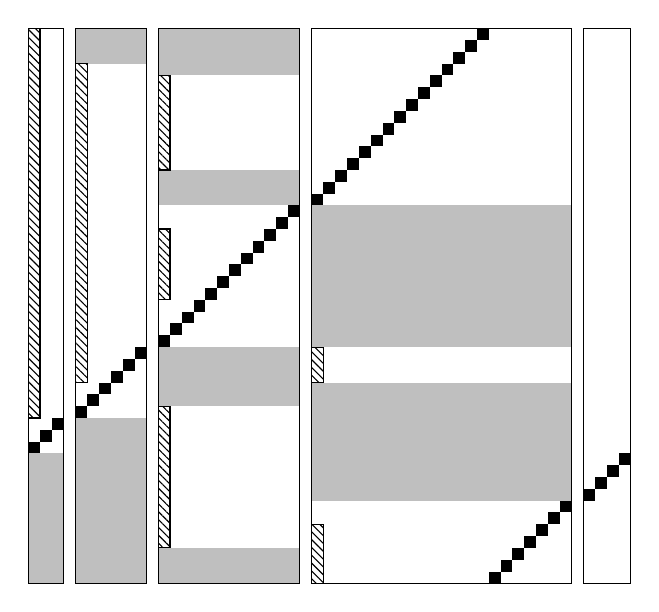
\begin{tikzpicture}
\begin{scope}[scale=0.15,every node/.style={align=center,scale=0.85}]
    % queries and high value buckets
    \fill[lightgray](0,-36) rectangle (3,-47);
    \fill[lightgray](4,0) rectangle (10,-3);
    \fill[lightgray](4,-33) rectangle (10,-47);
    \fill[lightgray](11,0) rectangle (23,-4);
    \fill[lightgray](11,-12) rectangle (23,-15);
    \fill[lightgray](11,-27) rectangle (23,-32);
    \fill[lightgray](11,-44) rectangle (23,-47);
    \fill[lightgray](24,-15) rectangle (46,-27);
    \fill[lightgray](24,-30) rectangle (46,-40);
    % queries
    \draw[pattern={Lines[angle=-45,distance=2pt]}](0,0) rectangle (1,-33);
    \draw[pattern={Lines[angle=-45,distance=2pt]}](4,-3) rectangle (5,-30);
    \draw[pattern={Lines[angle=-45,distance=2pt]}](11,-4) rectangle (12,-12);
    \draw[pattern={Lines[angle=-45,distance=2pt]}](11,-17) rectangle (12,-23);
    \draw[pattern={Lines[angle=-45,distance=2pt]}](11,-32) rectangle (12,-44);
    \draw[pattern={Lines[angle=-45,distance=2pt]}](24,-27) rectangle (25,-30);
    \draw[pattern={Lines[angle=-45,distance=2pt]}](24,-42) rectangle (25,-47);
    % cohorts
    \draw(0,0) rectangle (3,-47);
    \draw(4,0) rectangle (10,-47);
    \draw(11,0) rectangle (23,-47);
    \draw(24,0) rectangle (46,-47);
    \draw(47,0) rectangle (51,-47);
    % a hat = 36 alternative picked by the mechanism
    \foreach \i in {1,...,3}{
      \foreach \j in {1,...,3}{
        \fill[black](\i - 1,-36 +\i -1) rectangle (\i,-36 + \i);
      }
    }
    \foreach \i in {1,...,6}{
      \foreach \j in {1,...,6}{
        \fill[black](4 + \i - 1,-33 +\i -1) rectangle (4 + \i,-33 + \i);
      }
    }
    \foreach \i in {1,...,12}{
      \foreach \j in {1,...,12}{
        \fill[black](11 + \i - 1,-27 +\i -1) rectangle (11 + \i,-27 + \i);
      }
    }
    \foreach \i in {1,...,15}{
      \foreach \j in {1,...,15}{
        \fill[black](24 + \i - 1,-15 +\i -1) rectangle (24 + \i,-15 + \i);
      }
    }
    \foreach \i in {1,...,7}{
      \foreach \j in {1,...,7}{
        \fill[black](39 + \i - 1,-47 +\i -1) rectangle (39 + \i,-47 + \i);
      }
    }
    \foreach \i in {1,...,4}{
      \foreach \j in {1,...,4}{
        \fill[black](47 + \i - 1,-40 +\i -1) rectangle (47 + \i,-40 + \i);
      }
    }
\end{scope}
\end{tikzpicture}

\end{document}